\chapter{Implementering}

I dette kapitel vil der blive gennemgået forskellige dele af systemet.

\section{Kaldplan compiler}

Til at bygge en kaldplan er der lavet et bibliotek kaldet libdialplan der er skrevet i Dart. libdialplan er modellen for de kaldplaner som brugeren laver ude i klienten, i en struktur der efterligner hvad brugeren ser, for nemt at kunne genindlæse en kaldplan. Derfor har hvert komponent sin egen klasse i biblioteket, med en række felter svarende til de indstillinger som brugeren har for komponenten. Dette bibliotek genbruges i compileren, for dermed nemt at kunne indlæse den givende kaldplan i typestærke elementer.


Når en kaldplan er blevet bygget i klienten og gemt i databasen skal den oversættes til det format som Freeswitch forstår -- og til det bruges compileren. Når et opkald kommer ind i PBX'en går det ind i en context kaldet \enquote{public}, derfra skal opkaldet så sendes ud til den rette reception. Derfor er det første som compileren laver, at oprette en extension i \enquote{public} contextén hvorfra opkaldet bliver sendt ud til den pågældenes receptions context.
Ved at lave en context for hver reception, så giver det muligheden for at hvis der ikke er en extension der har alle sine conditions opfyldt og der ikke at lavet nogen anti-actions til at tage højde for det eller at der på andenvis er opstået en fejl i forbindelse med conditions, så kan man fordi den leder fra top til bund, placere i bunden en extension hvor dens condition altid er opfyldt \citep{minessale2012freeswitch}. Så hvis der for eksempel ikke er taget højde for et tidsinternal, så falder opkaldet til sidst altid ned i den. Det betyder også at der kun kan være en per context.

\section{Server}

Når en forespørgelse kommer ind til webserveren skal den først finde ud af hvilken resource som der spørges efter. Til det er biblioteket Route\footnote{Biblioteket kan hentes her http://pub.dartlang.org/packages/route} brugt som benytter sig af regulære udtryk til at viderstille forespørgelse til den rette funktion.
Route har mulighed for at man lave nogle filtre der tjekkes igennem først. Det er blevet udnyttet til at tjekke for om forespørgelse har en token og om den er gyldig til at verificere at de er logget ind. Hvis det er tilfældet så sendes forespørgelsen ud til den rette controller. 

Spørges der f.eks. efter at få oprette en ny reception, samler controllerne informationen sammen fra forespørgelsen og sender det til databasen der svare med id'et på den nye reception hvis det gik godt. Det id bliver så sendt tilbage til klienten igen.

\begin{figure}[ht!]
\centering
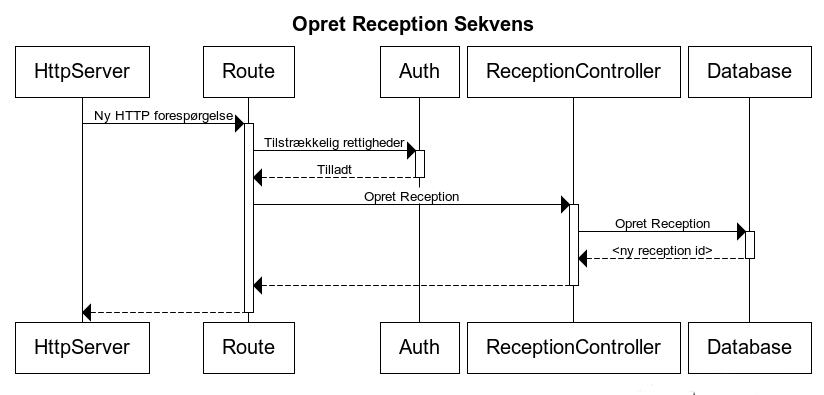
\includegraphics[width=\textwidth]{images/serversequence.png}
\caption{Når man kalder serveren for at oprette en ny reception}
\label{fig:serversequence}
\end{figure}

\pagebreak
\section{Migrering}
Når Responsum K/S skal lave skiftet til det nye system er det vigtigt at kunne få deres data med over. Til det er der blevet skrevet et lille program i Dart. Programmet er skrevet i Dart fordi modellen og forespørgelserne til databasen allerede var lavet i Dart, hvilket gjorder det hurtigt at låne der fra. Det gamle systems database var en Microsoft Access database og fordi at Dart ikke har support for at læse Access databaser blev der brugt et andet program \enquote{mdb-export} der gemmer tabellerne som kommasepareret filer. Migreringsprogrammet indlæser filerne til typestærke objekter og flytter det til felter i det nye databaseskema for så at gemme det i databasen.